
\documentclass[8pt, handout=show,notes=show]{beamer}

\usetheme{Boadilla}
\setbeamertemplate{blocks}[rounded][shadow=true]


%%%%lualatex on
%\usepackage{luatextra}
\usepackage{fontspec}
\usepackage{amsmath}
%Ligatures={Contextual, Common, Historical, Rare, Discretionary}
%\setmainfont[Mapping=tex-text]{Linux Libertine O}

\usepackage{natbib}
\usepackage{mathptmx}
\usepackage{latexsym}
\usepackage{mathtools}

\title{DACAS 1 -- 2016\\
	Models in Complex Systems
}

\date{Manchester, 2016}
\author{Simon Carrignon}

\begin{document}

\section{Build useful model}

\begin{frame}{Model to ``understand''}
	
	\begin{center}
		\includegraphics[width=.5\textwidth]{./fortGreekPlaceAndAmphora.png}
	\end{center}
	\begin{itemize}
		\item Collection of data:
			\begin{itemize}
				\item Why those data are distributed like that?
			\end{itemize}
	\end{itemize}
	\vfill
	$\rightarrow$ Model to understand what happened

\end{frame}

\begin{frame}
	What your model \emph{will explain}:\\
	\begin{itemize}
		\item general law,
		\item detailled description,
		\item ``de-idealization'' : make less and less abstraction. More precision, less generalization : 
	\begin{quote}
		``Model the size of the universe.''
	\end{quote}
	\end{itemize}
	\vfill
	\begin{alertblock}{Define precisely:}
		\begin{itemize}
			\item Questions at sake,
			\item Hypotheses tested,
			\item Assumption made,
			\item Avalaible data.
		\end{itemize}
	\end{alertblock}
	\vfil
	$\rightarrow$ Close relations between model and people that \emph{knows} about the system.
	\begin{quote}
		``To build a model helps to develop empathy \& understanding across a community.''\\
		\emph{(it is even mandatory)}
	\end{quote}


\end{frame}


\section{Ilustration}

\begin{frame}{Underlying code}
	\begin{center}
		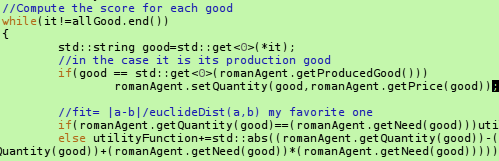
\includegraphics[width=1\textwidth]{./codePrices.png}\\
		\includegraphics[width=.4\textwidth]{./ClearingPriceDistanceEvolutionForTrade-G3N500.pdf}
	\end{center}
\end{frame}
\begin{frame}{}
	\begin{center}
		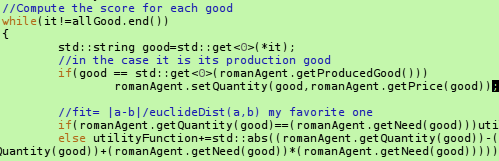
\includegraphics[width=1\textwidth]{./codePrices.png}\\
	\end{center}
\end{frame}

\begin{frame}
	\begin{center}

		\includegraphics[width=1\textwidth]{./codeNeeds.png}\\
	\end{center}
\end{frame}

\begin{frame}{Results}
	\begin{center}

		\includegraphics[width=1\textwidth]{./codeNeeds.png}\\
		\includegraphics[width=.4\textwidth]{./NonEquilibrium.png}
	\end{center}
\end{frame}


\end{document}
